% Options for packages loaded elsewhere
\PassOptionsToPackage{unicode}{hyperref}
\PassOptionsToPackage{hyphens}{url}
%
\documentclass[
  a4paper,
]{article}
\usepackage{lmodern}
\usepackage{amssymb,amsmath}
\usepackage{ifxetex,ifluatex}
\ifnum 0\ifxetex 1\fi\ifluatex 1\fi=0 % if pdftex
  \usepackage[T1]{fontenc}
  \usepackage[utf8]{inputenc}
  \usepackage{textcomp} % provide euro and other symbols
\else % if luatex or xetex
  \usepackage{unicode-math}
  \defaultfontfeatures{Scale=MatchLowercase}
  \defaultfontfeatures[\rmfamily]{Ligatures=TeX,Scale=1}
\fi
% Use upquote if available, for straight quotes in verbatim environments
\IfFileExists{upquote.sty}{\usepackage{upquote}}{}
\IfFileExists{microtype.sty}{% use microtype if available
  \usepackage[]{microtype}
  \UseMicrotypeSet[protrusion]{basicmath} % disable protrusion for tt fonts
}{}
\makeatletter
\@ifundefined{KOMAClassName}{% if non-KOMA class
  \IfFileExists{parskip.sty}{%
    \usepackage{parskip}
  }{% else
    \setlength{\parindent}{0pt}
    \setlength{\parskip}{6pt plus 2pt minus 1pt}}
}{% if KOMA class
  \KOMAoptions{parskip=half}}
\makeatother
\usepackage{xcolor}
\IfFileExists{xurl.sty}{\usepackage{xurl}}{} % add URL line breaks if available
\IfFileExists{bookmark.sty}{\usepackage{bookmark}}{\usepackage{hyperref}}
\hypersetup{
  hidelinks,
  pdfcreator={LaTeX via pandoc}}
\urlstyle{same} % disable monospaced font for URLs
\usepackage[left=3.8cm,right=2.5cm,top=2.5cm,bottom=2.5cm]{geometry}
\usepackage{graphicx,grffile}
\makeatletter
\def\maxwidth{\ifdim\Gin@nat@width>\linewidth\linewidth\else\Gin@nat@width\fi}
\def\maxheight{\ifdim\Gin@nat@height>\textheight\textheight\else\Gin@nat@height\fi}
\makeatother
% Scale images if necessary, so that they will not overflow the page
% margins by default, and it is still possible to overwrite the defaults
% using explicit options in \includegraphics[width, height, ...]{}
\setkeys{Gin}{width=\maxwidth,height=\maxheight,keepaspectratio}
% Set default figure placement to htbp
\makeatletter
\def\fps@figure{htbp}
\makeatother
\setlength{\emergencystretch}{3em} % prevent overfull lines
\providecommand{\tightlist}{%
  \setlength{\itemsep}{0pt}\setlength{\parskip}{0pt}}
\setcounter{secnumdepth}{5}
\usepackage{amsmath} \usepackage{pdflscape} \usepackage{array} \usepackage{multirow}

\author{}
\date{\vspace{-2.5em}}

\begin{document}

\pagenumbering{roman}

\newpage

\begin{center}          % <!-- center text -->

\LARGE{Cyclist Road Accidents in UK using Machine Learning and Visualization techniques.} % <!-- make large text -->

\bigskip                % <!-- blank lines -->
\bigskip


\begin{center}\includegraphics[width=4.28in]{university logo} \end{center}

\large{A thesis presented for the degree of }

\large{MSc. Data Science and Analytics} 

------------------------------------------------

\large{Submitted by}



\LARGE{Suraj Sankar Mandal}

\LARGE(19251248)

\bigskip
\bigskip

\large{under the guidance of the supervisor}


\LARGE{Dr. Catherine Hurley}

\bigskip
\bigskip
\bigskip
\bigskip

\large{Department of Mathematics and Statistics}

\large{Maynooth University}

\large{August 2020}



\end{center}

\newpage

\begin{center}

\LARGE{STATEMENT OF ORIGINALITY}
 

\end{center}

\bigskip

I have read and accepted the Departmental policies on plagiarism and
acknowledge that the work presented in this study entitled Cyclist Road
Accidents in the United Kingdom using Machine Learning and Visualization
Technology is my own and has not been applied in any way to any degree
or qualification at any university or other tertiary institution. In
addition, I have referenced correctly all literature and sources used in
this work.

\textbf{Signed by: } Suraj Mandal

\textbf{Date: } 13/08/2020

\newpage

\begin{center}

\LARGE{ACKNOWLEDGEMENT}
 

\end{center}

I would like to convey my heartfelt gratitude to my supervisor,
\textbf{Dr.~Catherine Hurley}, for her tremendous encouragement and
dedication to supporting me through the entire process. Her guidance,
assistance and inspiration encouraged me to finish the project. I am
thankful to my supervisor for arranging weekly team sessions, discussing
my concerns and recommending opportunities to strengthen the research
process.

\newpage

\begin{center}

\large{Abstract}



\end{center}

\bigskip

Road Traffic Accidents (RTAs) are a major problem in today's world, as
their number continues to grow every year due to an increase in the use
of road transport and a variety of other factors. All datasets were
imported from traffic incidents, taken from the UK dataset STATS19 for
the year 2018. The knowledge derived from these large datasets forms the
basis for a variety of predictions. Some data mining methods, such as
the handling of an imbalanced dataset, Naive Bayes, Logistic Regression,
Random Forest and Decision Tree, are used for prediction purposes. This
paper describes the best algorithm model to be used to improve the
accuracy and predictability of cyclist accidents. The project will
define the most suitable classification algorithm that can be used to
predict cyclist casualties in the future. In addition, the key factors
causing these road accidents are identified and presented.

\textbf{Keywords--- } Road Accident, Naive Bayes, Logistic Regression,
Random Forest, Decision Tree.

\newpage

\tableofcontents

\newpage

\hypertarget{list-of-tables}{%
\section*{List of tables}\label{list-of-tables}}
\addcontentsline{toc}{section}{List of tables}

\renewcommand{\listtablename}{}
\listoftables

\newpage

\hypertarget{list-of-figures}{%
\section*{List of figures}\label{list-of-figures}}
\addcontentsline{toc}{section}{List of figures}

\renewcommand{\listfigurename}{}
\listoffigures

\newpage

\pagenumbering{arabic}

\hypertarget{intro}{%
\section{Introduction}\label{intro}}

\hypertarget{purpose-and-motivation}{%
\subsection{Purpose and Motivation}\label{purpose-and-motivation}}

Road Traffic Accidents (RTAs) are one of the primary causes of death in
today's world, ranking as the 10th leading cause of death worldwide.
Road safety is a critical issue for many countries, where traffic deaths
and injuries are increasingly recognized as a significant public health
problem. According to the World Health Organization (WHO), nearly 1.25
million people die per year in traffic accidents, with an average of
3,287 deaths each day. In comparison, traffic fatalities rate as the 9th
leading cause of death and account for 2.2\% of all deaths worldwide. By
analyzing these factors and making effective predictions using data
mining techniques, proper precautions can be taken to minimize the
severity of these cyclist casualties. In the United Kingdom, the number
of miles cycled per person seems to have increased from 37 to 53 miles
in recent years (DfT, 2013). In the United Kingdom, the risk of death
from traveling one kilometer on foot or by bicycle is more than 17 times
higher than that of a car (Davies, 2014). The geographical and
demographic distribution of factors linked to the uptake of bicycles has
powerful policy implications, but has received little academic attention
(Fraser \& Lock, 2011). As a big data project, I wanted to use machine
learning to explore the factors affecting cyclist accidents in more
detail.

\hypertarget{about-the-dataset}{%
\subsection{About the dataset}\label{about-the-dataset}}

The following three datasets were used for research purposes and were
collected from the UK dataset STATS19 (2018) in R(Lovelace et al.
(2019)) which is available at data.gov.uk (Safety (2018)). The data are
collected by the police at the roadside, the variables and fields
collected are defined by the Department for Transport (DfT) and these
have been agreed by the Standing Committee for Road Accident Statistics
(SCRAS) and Association of Chief Police Officers (ACPO). The three
datasets `Accidents,' `Casualties' and `Vehicles' were merged together
into a single dataset used for the analysis and modeling of data in this
study. The merged data set consists of 160,597 observations and 68
variables. The dataset provides information on the geographical area of
the accident, road conditions, light conditions, weather conditions,
severity of the accident, casualties and vehicle make and type. The
target variable for the prediction is the `Casualty Severity', which is
a factor variable that contains three levels such as `fatal', `serious',
and `slight' for `Casualty Type' - cyclist. The remaining 67 independent
variables will provide information on the target variable predictions.

\hypertarget{aims-and-objectives}{%
\subsection{Aims and Objectives}\label{aims-and-objectives}}

The aims and objectives of this project are as follows:

\begin{itemize}
\item
  \textbf{Objective A:} Identify the main factors that have a
  significant effect on cyclist accidents in United Kingdom.
\item
  \textbf{Objective B:} To implement and evaluate the following
  classification models and to evaluate their results in order to
  identify the most efficient algorithm.

  \begin{itemize}
  \tightlist
  \item
    Naive Bayes
  \item
    Logistic Regression
  \item
    Random Forest
  \item
    Decision Tree
  \end{itemize}
\item
  \textbf{Objective C:} To demonstrate ways of handling an imbalanced
  data.
\item
  \textbf{Objective D:} Identifying the important attributes of the data
  using Random Forest technique and feeding the important ones as input
  to other classification techniques to identify if it yields better
  results than the existing models.
\end{itemize}

\hypertarget{outline-of-the-thesis}{%
\subsection{Outline of the Thesis}\label{outline-of-the-thesis}}

This thesis has been structured into five chapters and each chapter has
multiple subsections.

\emph{Chapter 1: Introduction}

Provides an introduction to the research topic with aim and objectives
of the project and provides an overview to different chapters in the
thesis.

\emph{Chapter 2: Background}

Highlights the similar work performed in literature.

\emph{Chapter 3: Methodology}

This chapter explains the detailed methodology implemented in the
analysis of datasets.

\emph{Chapter 4: Results}

Demonstrates the results obtained after analysis of dataset.

\emph{Chapter 5: Conclusion and Future Scope}

Concludes the results obtained from this project and discusses the
future scope of this project.

\newpage

\hypertarget{background}{%
\section{Background}\label{background}}

\hypertarget{literature-review}{%
\subsection{Literature Review}\label{literature-review}}

The main focus of earlier studies identified various attributes, such as
road segments, intersections, road surfaces and weather, which have a
significant impact on crashes. This has led to a number of improvements
in road safety measures. Despite the attributes mentioned above, it can
not be the main contributor to the crash. Few researchers have studied
the properties of macro-levels such as cross junction, traffic zones,
census. There are a significant number of unobserved explanatory
variables in road crash analyzes that influence the frequency and
severity of accidents. Identifying the hidden pattern is quite a
challenge. The reason for most of the accident data is highly
imbalanced, which makes the analysis quite challenging. Traditionally,
road accident hotspot analysis has focused on road segments or specific
junctions, while area-wide hotspots and the spread of risk resulting
from a collision are somewhat neglected. The methodological downside was
that Poisson log linear regression was used to compensate for the
randomness of time and space incidents (Daniel Blower (1993)). In a
joint (Rami Harb (2009)) analysis, the causality of the accident was
investigated using the Random forest and the decision tree. This helped
to classify the location of the vehicles, and the driver characteristics
of the accident avoidance maneuvers result were more reliable compared
to the genetic algorithm. A two-stage mixed multivariate model to
estimate the occurrence of incidents at their severity rates, which
helped classify the low-frequency accident. (Sowmya and
Ponmuthuramalingam (2013)) predicted the causality severity of the
accident using Naive Bayes model technique. The accuracy of the the
model was comparatively high than other models. The author (Brennan
(2012)) studied the data imbalance class using various tools and methods
to produce accurate results. Data imbalance is a major issue in the
approach to data mining, the author has provided a very extensive
approach to dealing with class imbalances using boosting and other
techniques.

\newpage

\hypertarget{methodology}{%
\section{Methodology}\label{methodology}}

\hypertarget{crisp-dm-methodology}{%
\subsection{CRISP-DM methodology}\label{crisp-dm-methodology}}

Cross-industry Standard Process for Data Mining (CRISP-DM) is being used
in the project. Based on the polls of the KDNuggets, CRISP-DM is one of
the common methodologies that comes with six different phases. The
phases are business understanding, data understanding, data preparation,
modeling, evaluation and deployment. The following (figure 1) shows the
CRISP-DM Methodology.

\begin{figure}[h!]

{\centering 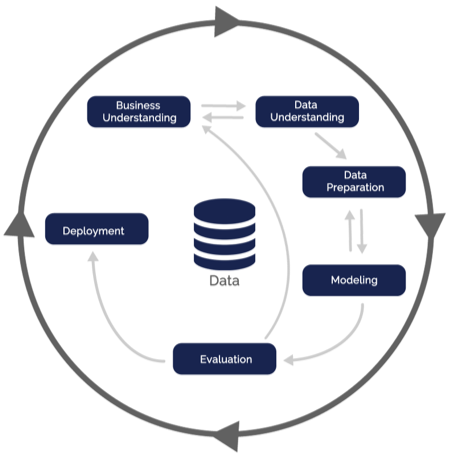
\includegraphics[width=6.31in]{crisp-dm} 

}

\caption{CRISP-DM Methodology}\label{fig:unnamed-chunk-2}
\end{figure}

\begin{itemize}
\item
  \textbf{Phase-1 Business Understanding:} The first step involves doing
  a critical review on cyclist accidents which occurred in United
  Kingdom. The objective is to support authorities in the improving the
  road networks.
\item
  \textbf{Phase-2 Data Understanding:} The data needed to conduct the
  cyclist road accident analysis in the United Kingdom were collected
  from the UK dataset STATS19 (2018)(Lovelace et al. (2019)). The
  repository consists of three files relating to accidents, casualties
  and vehicles in the .csv format, which are combined together into one
  for data analysis. The extracted data was evaluated to ensure that it
  met the business requirements with the aid of a data description
  guide. The merged dataset comprises of 160,597 observations and 68
  variables including the target variable, `Casualty Severity'. Some of
  the attributes are as follows.

  \begin{itemize}
  \item
    \emph{Police\_Force} : Types of police forces in United Kingdom
    which consists of 51 classes for counties.
  \item
    \emph{Casualty\_Severity} : Severity of the accidents occurred for
    the casualty type cyclist. This is the target variable for this
    study. It consists of three classes such as slight, serious and
    fatal.
  \item
    \emph{Date} : It shows the date on which the accident occurred.
  \item
    \emph{Day\_of\_Week} : The occurrence of an accident on a particular
    day of the week.
  \item
    \emph{Time} : Accidental occurrence at various times.
  \item
    \emph{Local\_Authority\_District} : The authority concerned for the
    particular district in which the accident occurred. Variable has 416
    classes comprising all regions of the United Kingdom.
  \item
    \emph{Road\_Type} : Denotes the type of road. It has 8 classes.
  \item
    \emph{Speed\_limit} : It denotes the speed limit set for the roads
    where the casualties happened.
  \item
    \emph{Junction\_Detail} : This provides details on the respective
    junctions at which accidents occurred. It contains 10 classes.
  \item
    \emph{Light\_Conditions} : This denotes the light conditions at the
    event of accidents. It contains 6 classes.
  \item
    \emph{Weather\_Conditions} : It denotes the weather conditions
    during which the accidents occurred. It contains 10 classes.
  \item
    \emph{Road\_Surface\_Conditions} : It denotes the surface conditions
    of the roads in which accidents have occurred. It contains 7
    classes.
  \item
    \emph{Urban\_or\_Rural\_Area} : It indicates whether the accident
    occurred in urban or rural areas. It contains 3 classes.
  \item
    \emph{Age\_of\_Casualty} : This indicates the age of the casualties
    at the time of the accident.
  \item
    \emph{Sex\_of\_Casualty} : It denotes the gender of the casualty.
  \item
    \emph{Journey\_Purpose\_of\_Driver} : It denotes the journey purpose
    of the driver. It consists of 6 classes.
  \item
    \emph{Special\_Conditions\_at\_Site} : It denotes if there were any
    special conditions at the site. It contains 9 classes.
  \item
    \emph{Junction\_Control} : It contains information about the
    respective individual/thing who is in charge of the respective
    junction in which accidents occurred. It contains 6 classes.
  \end{itemize}
\item
  \textbf{Phase-3 Data Preparation:} It consists of integration and
  cleaning of data. For this project, the three.csv files are merged
  together using the RStudio merge feature.
\item
  \textbf{Phase-4 Data Modeling:} This step consists of implementing
  method that uses various data mining algorithms,i.e.~naive
  bayes,Logistic Regression, random forest and decision tree algorithms
  to implement the predictive models and the ROSE package is used to
  manage the imbalanced data collection.
\item
  \textbf{Phase-5 Data Evaluation:} This step consists of data
  evaluation of the results for the predictive models. In this project
  metrics such as confusion matrix and accuracy are used to determine
  the best-fit algorithm.
\item
  \textbf{Phase-6 Data Deployment:} This is the final step of the
  CRISP-DM Methodology, R-studio was used to deploy an algorithm that
  provides the highest accuracy for constructing the model and
  predicting the extent of cyclist accidents in the United Kingdom.
\end{itemize}

\hypertarget{data-preparation}{%
\subsection{Data Preparation}\label{data-preparation}}

The data needed to conduct the cyclist accident analysis in the United
Kingdom were collected from the UK dataset STATS19 (2018) (Lovelace et
al. (2019)). Initial data collection includes gathering datasets, as the
repository consists of three files `accident.csv' , `vehicle.csv' and
`casualty.csv' for the year 2018. Every of these reports includes the
necessary information on road collisions, their victims and the vehicles
involved. These three files are loaded into the RStudio and merged into
a single csv file based on their respective `accident index' using the R
programming `merge' function. To look for the cyclist casualty the
author have filter the dataset using the filter function from tidyverse
package in R(Wickham et al. (2019)) where the Casualty Type is
`Cyclist'. As a result, the data set for the analysis of this study is
produced.

\begin{figure}[h!]

{\centering 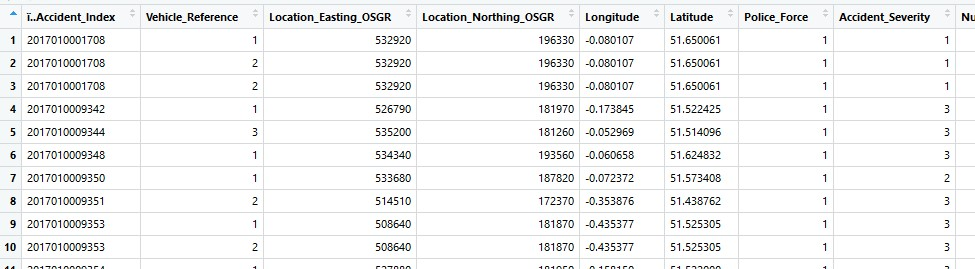
\includegraphics[width=13.54in,height=0.16\textheight]{figure 1} 

}

\caption{Snapshot of the merged dataset}\label{fig:unnamed-chunk-3}
\end{figure}

(Figure 2) provides a snapshot of the combined dataset for our study,
consisting of a total of 68 variables and 17550 observations.

\hypertarget{treating-the-missing-values}{%
\subsubsection{Treating the missing
values}\label{treating-the-missing-values}}

It is important to treat the missing values in the dataset as they
affect the accuracy of the prediction during modeling and provide
incorrect results. There are about 32 missing values in this dataset.
Upon further study , it was noted that several instances had a value of
`-1' which was also considered missing as per the data guide obtained.
As a result, instances containing the value `-1' were replaced by `NA'
using the `lapply'(Bengtsson (2020)) function (figure 3) so that they
could be viewed as missing values. This resulted in a few instances of
missing values in the results. Omit function in R(Dowle and Srinivasan
(2019)) was used to remove all the missing values and the dataset with
no missing values was thus obtained for further analysis.

\begin{figure}[h!]

{\centering 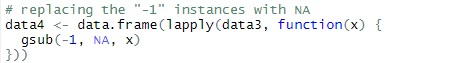
\includegraphics[width=0.75\linewidth]{figure 3} 

}

\caption{Replacing the '-1' with 'NA'}\label{fig:unnamed-chunk-4}
\end{figure}

\hypertarget{selecting-the-desired-variables}{%
\subsubsection{Selecting the desired
variables}\label{selecting-the-desired-variables}}

Using too many variables on the dataset while modeling makes the process
difficult and reduces the performance of the predictions due to the
effect of irrelevant attributes. The dataset includes 68 attributes,
most of which are not applicable to the subject area of this report,
such as vehicle registration number, propulsion code,
engine\_capacity\_cc, location easting of OSGR, engine\_capacity\_cc,
location northing of OSGR, was\_vehicle\_left\_hand\_drive etc. Thus,
the irrelevant attributes have been deleted and refined to include only
the following 16 main variables (Table 1) that affect the target
variable `Casualty Severity' for cyclist.

\begin{table}[!htb]
\caption{Selected attributes from the whole dataset}
\bigskip
\centering
\begin{tabular}{c l}
\hline\hline
Serial no. & Names of Attribute\\ [0.75ex]
\hline
1 & Date  \\
2 & Day\_of\_Week \\
3 & Time \\
4 & Road\_Type \\
5 & Speed\_limit  \\
6 & Junction\_Detail \\
7 & Junction\_Control \\
8 & Light\_Conditions \\
9 & Weather\_Conditions  \\
10 & Road\_Surface\_Conditions \\
11 & Special\_Conditions\_at\_Site \\
12 & Urban\_or\_Rural\_Area \\ 
13 & Sex\_of\_Casualty  \\
14 & Age\_of\_Casualty \\
15 & Casualty\_Severity \\
16 & Journey\_Purpose\_of\_Driver \\ [1ex]
\hline
\end{tabular}
\label{tab:Table 1}
\end{table}

\newpage

\hypertarget{treating-the-class-variables}{%
\subsubsection{Treating the class
variables}\label{treating-the-class-variables}}

In the current dataset, the class of several variables was incorrect and
was given by default as character as shown in (Table 2).

\begin{table}[h]
\caption{Structure of the dataset displaying the class of each variable}
\bigskip
\centering
\begin{tabular}{l l}
\hline\hline
Names of Attribute & Class of variables\\ [0.75ex]
\hline
Date & chr  \\
Day\_of\_Week & chr \\
Time & chr \\
Road\_Type & chr \\
Speed\_limit & chr  \\
Junction\_Detail & chr \\
Junction\_Control & chr \\
Light\_Conditions  & chr\\
Weather\_Conditions   & chr\\
Road\_Surface\_Conditions  & chr\\
Special\_Conditions\_at\_Site  & chr\\
Urban\_or\_Rural\_Area  & chr\\ 
Sex\_of\_Casualty   & chr\\
Age\_of\_Casualty  & chr\\
Casualty\_Severity  & chr\\
Journey\_Purpose\_of\_Driver & chr \\ [1ex]
\hline
\end{tabular}
\label{tab:Table 2}
\end{table}

As shown in Table 2, all the variables such as age of casualty, date and
time variable, day of week, etc. are incorrectly classified as
characters which is incorrect. Identifying the right class of each
variable and converting it to the required class was then carried out.

\begin{table}[h]
\caption{Structure of the dataset showing the appropriate class and the levels for variables}
\bigskip
\centering
\begin{tabular}{l l}
\hline\hline
Names of Attribute & Class of variables\\ [0.75ex]
\hline
Date &  Factor w/ 12 levels  \\
Day\_of\_Week & Factor w/ 7 levels \\
Time & Factor w/ 4 levels \\
Road\_Type & Factor w/ 6 levels \\
Speed\_limit & Factor w/ 6 levels  \\
Junction\_Detail & Factor w/ 8 levels \\
Junction\_Control & Factor w/ 4 levels \\
Light\_Conditions  & Factor w/ 3 levels\\
Weather\_Conditions   & Factor w/ 8 levels\\
Road\_Surface\_Conditions  & Factor w/ 5 levels\\
Special\_Conditions\_at\_Site  & Factor w/ 8 levels\\
Urban\_or\_Rural\_Area  & Factor w/ 3 levels\\ 
Sex\_of\_Casualty   & Factor w/ 2 levels\\
Age\_of\_Casualty  & int\\
Casualty\_Severity  & Factor w/ 3 levels\\
Journey\_Purpose\_of\_Driver & Factor w/ 3 levels \\ [1ex]
\hline
\end{tabular}
\label{tab:Table 3}
\end{table}

\bigskip
\newpage

Table 3 demonstrates that all variables are organized into the dataset
with the correct classes and levels.

\hypertarget{binning-the-factor-variables}{%
\subsubsection{Binning the factor
variables}\label{binning-the-factor-variables}}

Binning the levels in a factor variable involves in combining several
levels into one for better data analysis and increasing the uniqueness
of each level. The following levels of the variables are binned
accordingly for an effective analysis.

\begin{figure}[h!]

{\centering 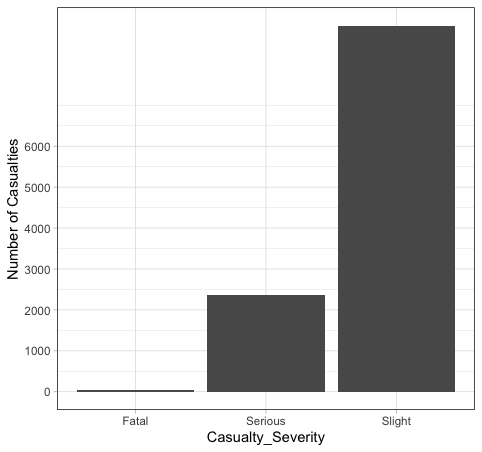
\includegraphics[width=0.75\linewidth]{cas} 

}

\caption{Distribution of the target variable}\label{fig:unnamed-chunk-5}
\end{figure}

\begin{itemize}
\item
  The target variable, `Casualty Severity' consists of 3 levels:
  `Fatal', `Serious', `Slight'. However, the data is imbalanced as shown
  in (figure 4), as a result, the target variable is biased towards the
  class `Slight' with 80\% of data. Hence, the two levels `Fatal' and
  `Serious' are combined into one level as `High', while the other
  majority class as `Low'.
\item
  The `time' variable consists of time-stamps of the accident
  occurrence. In order to make this more meaningful and useful, the
  variable is converted into a factor variable containing 4 levels:
  `Morning (5-12)', `Afternoon (12-17)', `Evening (17-20)', and `Night
  (20-5)'.
\item
  The `light conditions' with 5 levels were shrunk to 3 levels: `Lit',
  `Dark', `Unknown'.
\item
  The `weather conditions' with 9 levels were reduced to 8 levels: `Fine
  -- no high winds', `Rain -- no high winds', `Snow -- no high winds',
  `Fine -- high winds', `Rain -- high winds', `Snow -- high winds',
  `Fog/Mist', `Other'.
\item
  The variable, `Journey purpose of driver' with 7 levels were reduced
  to 3 levels: `For work', `For school', `Other'.
\item
  The variable, `Road surface conditions' was categorized into 7 levels:
  `Dry', `Wet/Damp', `Snow', `Frost/Ice', `Flood (3cm. deep)',
  `Oil/Diesel', `Mud'.
\item
  The variable, `Day of the week' was simply classified into `Monday',
  `Tuesday', `Wednesday', `Thursday', `Friday', `Saturday', and
  `Sunday'.
\item
  The variable, `Road type' was classified into `Roundabout', `One way
  street', `Dual carriageway', `Single carriageway', `Slip road',
  `Unknown'.
\end{itemize}

With the implementation of all the above-mentioned changes, the refined
dataset's structure is as follows (Table 4).

\begin{table}[h]
\caption{Structure of the refined dataset after binning the levels of factor variables}
\bigskip
\centering
\begin{tabular}{l l l}
\hline\hline
Names of Attribute & Class of variables & Levels\\ [0.75ex]
\hline
Date & Date  & format: '01/01/2018',..\\
Day\_of\_Week & Factor w/ 7 levels & 'Sunday','Monday',...\\
Time & Factor w/ 4 levels & 'Night','Morning',...\\
Road\_Type & Factor w/ 6 levels & 'Roundabout', 'One way street',...\\
Speed\_limit & Factor w/ 6 levels  & '20','30','40',...\\
Junction\_Detail & Factor w/ 8 levels & 'Roundabout','Mini-roundabout'\\
Junction\_Control & Factor w/ 4 levels & 'Authorised person','Auto traffic signal',...\\
Light\_Conditions  & Factor w/ 3 levels & 'Lit', 'Dark',...\\
Weather\_Conditions   & Factor w/ 8 levels & 'Fine – no high winds', 'Rain – no high winds',...\\
Road\_Surface\_Conditions  & Factor w/ 5 levels & 'Dry', 'Wet/Damp',...\\
Special\_Conditions\_at\_Site  & Factor w/ 8 levels & 'None','Auto traffic signal - out',...\\
Urban\_or\_Rural\_Area  & Factor w/ 3 levels & 'Urban','Rural,...\\ 
Sex\_of\_Casualty   & Factor w/ 2 levels & 'Male','Female',...\\
Age\_of\_Casualty  & int &  27 35 31 19 23 40 31 25 49 42 ...\\
Casualty\_Severity  & Factor w/ 3 levels & 'High','Low'\\
Journey\_Purpose\_of\_Driver & Factor w/ 3 levels & 'For work', 'For school',...\\ [1ex]
\hline
\end{tabular}
\label{tab:Table 4}
\end{table}

\newpage

\hypertarget{data-exploration}{%
\subsection{Data Exploration}\label{data-exploration}}

Data exploration is one of the stages in which data is analyzed and
visualized using R. Distribution of all attributes is analyzed here to
recognize trends and patterns.

\begin{figure}[h!]

{\centering 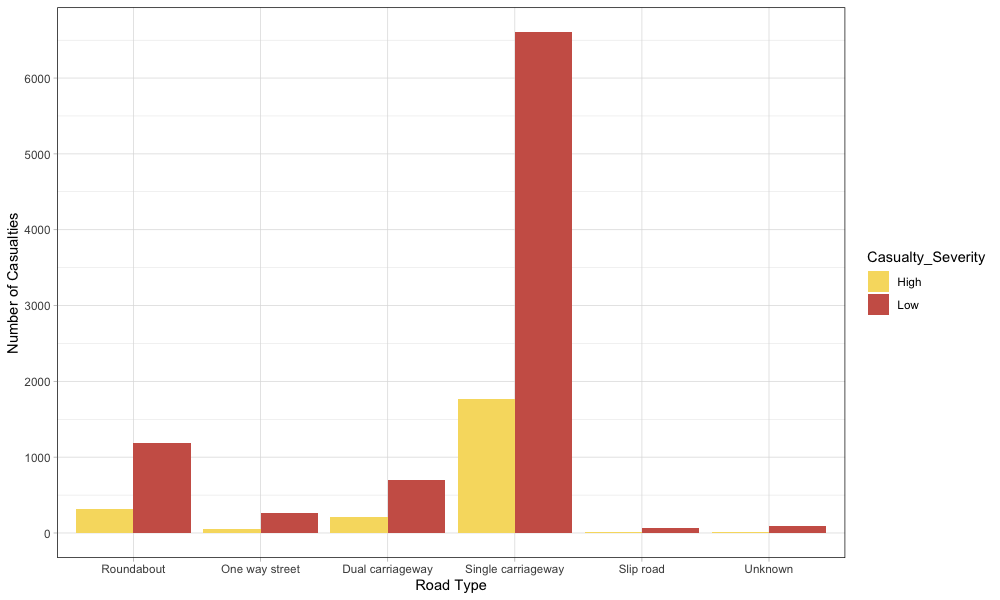
\includegraphics[width=0.75\linewidth]{rt} 

}

\caption{Casualty type counts by road type}\label{fig:unnamed-chunk-6}
\end{figure}

(Figure 5) indicates the occurrence of accidents on the basis of a road
type. It is quite clear from the data shown that the majority of
casualties occurred on single carriageway. The second row is roundabout
roadtype. One way street seems to be far safe with very less occurrences
of cyclist casualties.

\begin{figure}[h!]

{\centering 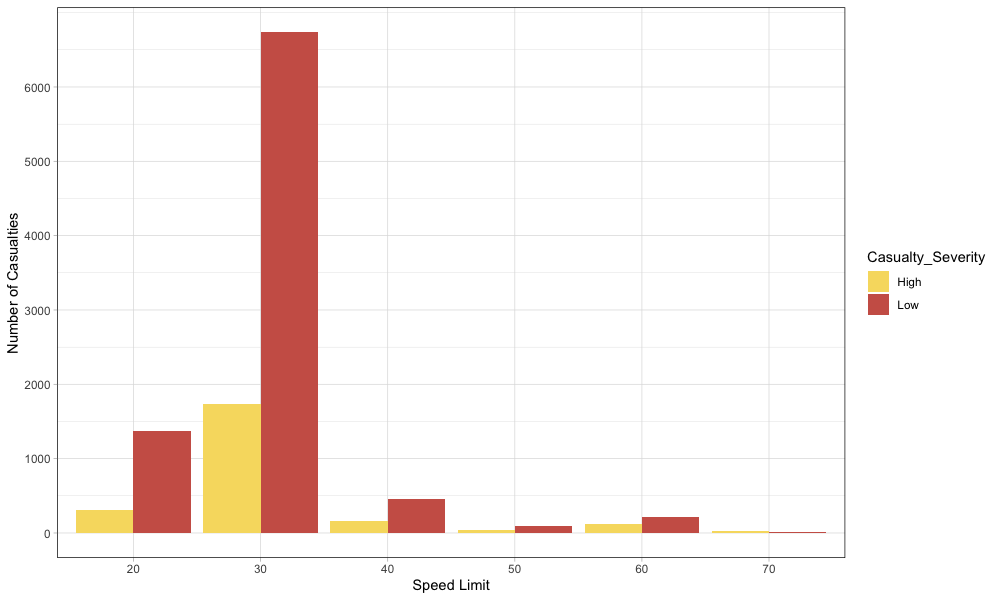
\includegraphics[width=0.75\linewidth]{sl} 

}

\caption{Casualty type counts by speed limit}\label{fig:unnamed-chunk-7}
\end{figure}

(Figure 6) indicates the number of casualties that occurred at each set
of speed limit. It is clear from the figure shown that most of the
incidents happened on roads where the speed limit was to be just 30 mph.
It gives rise to concerns that incidents may have occurred on such roads
due to over-speeding of vehicles at 30 mph is perceived to be a
reasonable speed limit.

\newpage
\begin{figure}[h!]

{\centering 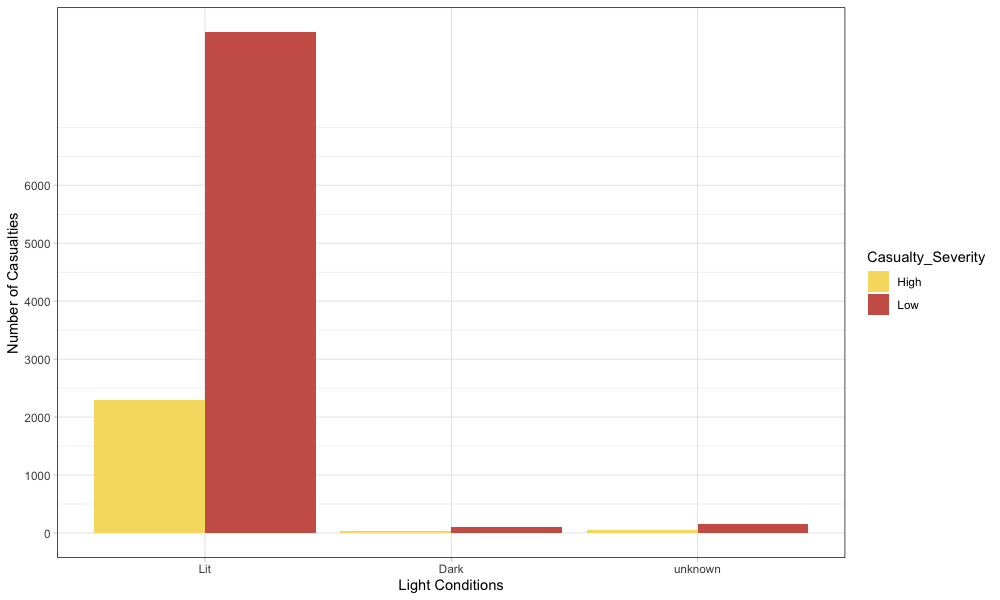
\includegraphics[width=0.75\linewidth]{lc} 

}

\caption{Casualty type counts by light conditions}\label{fig:unnamed-chunk-8}
\end{figure}

(Figure 7) indicates the frequency of injuries under various light
conditions. Contrary to the assumption that casualties are more likely
to occur under dark conditions, evidence indicates that most injuries
have occurred under well-lit conditions.

\begin{figure}[h!]

{\centering 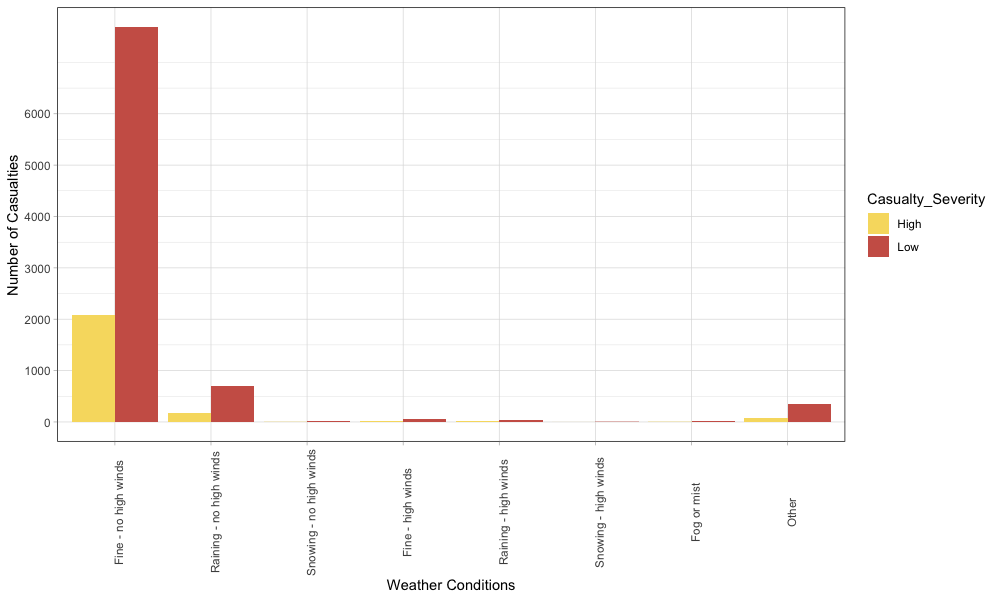
\includegraphics[width=0.75\linewidth]{wc} 

}

\caption{Casualty type counts by weather conditions}\label{fig:unnamed-chunk-9}
\end{figure}

(Figure 8) indicates the distribution of injuries occurring in various
environmental conditions. As most injuries have happened in good weather
conditions with no strong winds, opposed to bad weather conditions such
as high winds, rain, snow, etc

\begin{figure}[h!]

{\centering 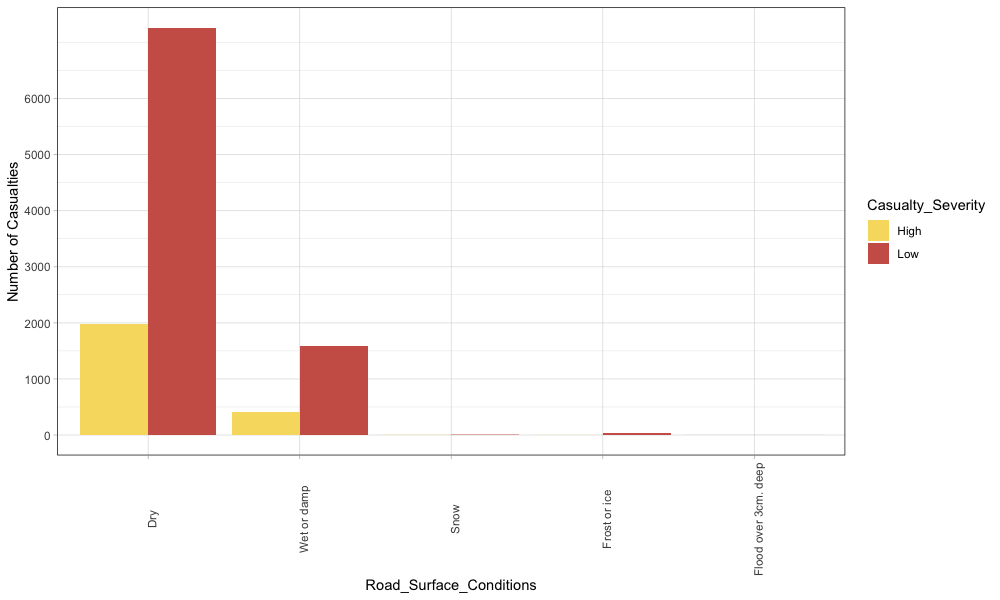
\includegraphics[width=0.75\linewidth]{rs} 

}

\caption{Casualty type counts by road surface conditions}\label{fig:unnamed-chunk-10}
\end{figure}

\newpage

(Figure 9) indicates the road surface conditions in which casualties
have occurred. Although most of the casualties took place under dry road
conditions, some casualties occurred under wet road conditions.

\begin{figure}[h!]

{\centering 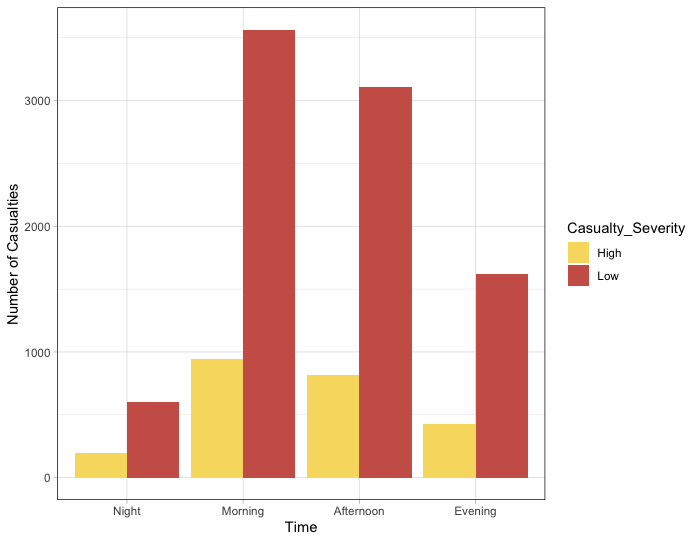
\includegraphics[width=0.75\linewidth]{time} 

}

\caption{Casualty type counts by time}\label{fig:unnamed-chunk-11}
\end{figure}

(Figure 10), displays the time variable distribution. Contrary to the
belief that most of the casualties may have happened during night hours,
data shows that most of the casualties occurred in daylight conditions
during the morning /afternoon period.

\newpage
\begin{figure}[h!]

{\centering 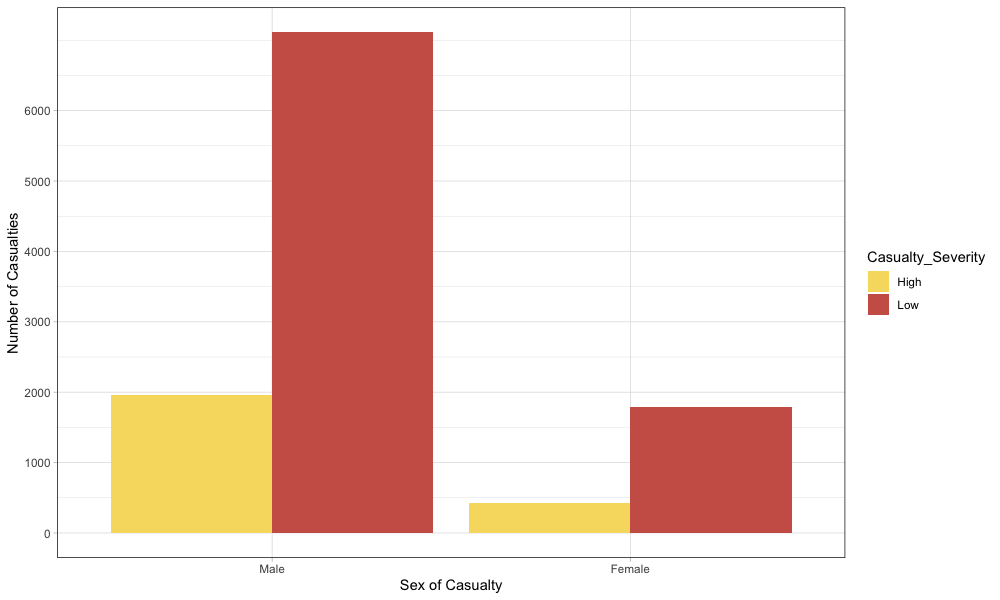
\includegraphics[width=0.75\linewidth]{sc} 

}

\caption{Casualty type counts by gender}\label{fig:unnamed-chunk-12}
\end{figure}

(Figure 11), displays the casualties based on gender. As shown in the
figure 80\% of male cyclist are prone to casualties compare to female
cyclist.

\begin{figure}[h!]

{\centering 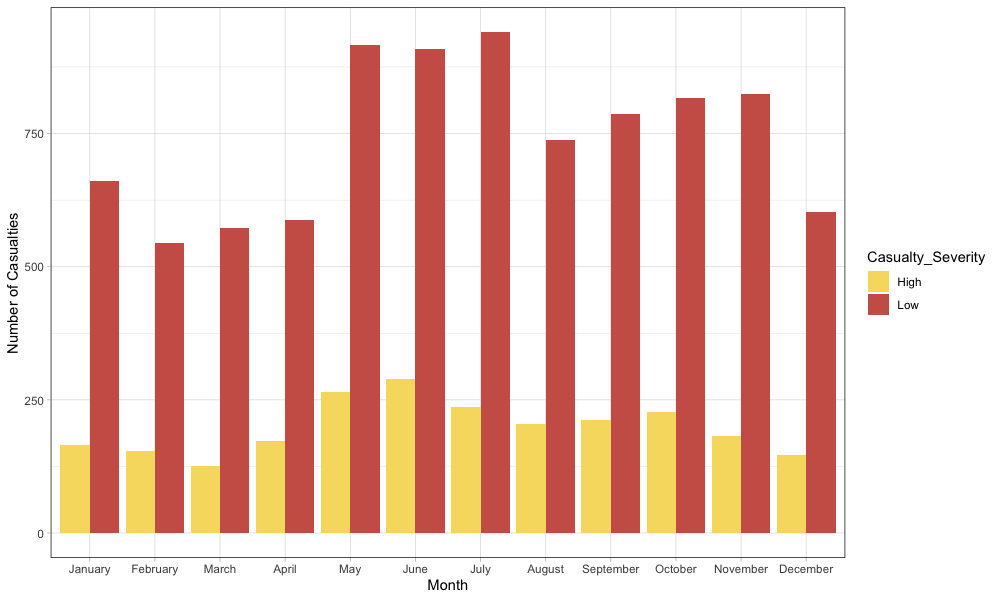
\includegraphics[width=0.75\linewidth]{date} 

}

\caption{Casualty type counts by month}\label{fig:unnamed-chunk-13}
\end{figure}

(Figure 12), shows the monthly casualties. As shown in the figure, the
number of casualties occurs every month but more casualties can be seen
in May, June and July compared to other months.

\newpage
\begin{figure}[h!]

{\centering 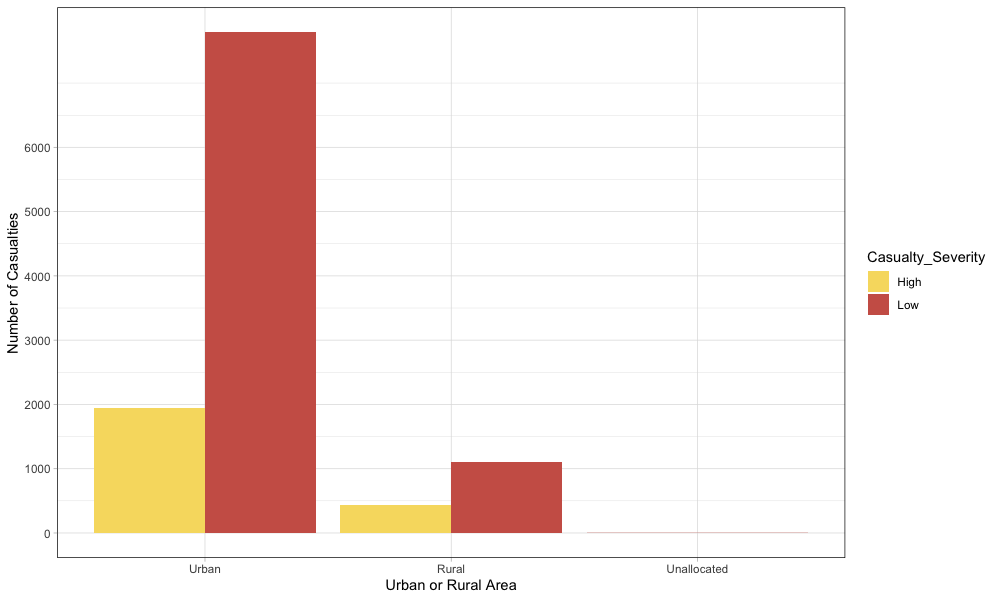
\includegraphics[width=0.75\linewidth]{ur} 

}

\caption{Casualty type counts by urban or rural area}\label{fig:unnamed-chunk-14}
\end{figure}

(Figure 13), shows the number of casualties in the urban or rural areas.
The number of casualties, as shown in the figure, is more in urban areas
compared to rural areas.

\begin{figure}[h!]

{\centering 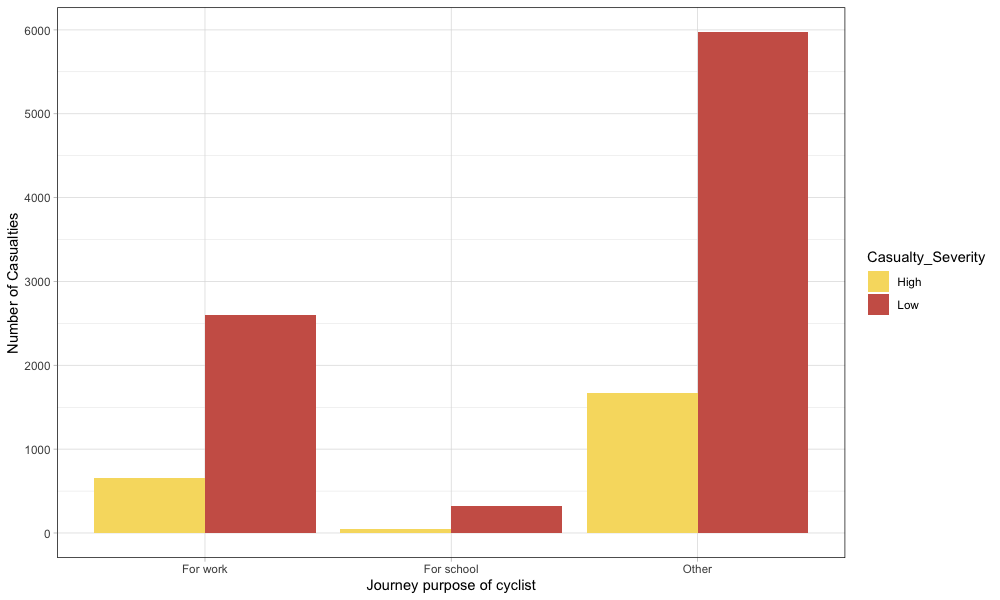
\includegraphics[width=0.75\linewidth]{jpc} 

}

\caption{Casualty type counts by journey purpose of cyclist}\label{fig:unnamed-chunk-15}
\end{figure}

(Figure 14), shows casualties based on cyclist's journey purpose. As
shown in the figure, the number of casualties occurred while the cyclist
was out for other work on the road and the least casualties occurred
whilst the cyclist was off to school.

\hypertarget{data-modeling}{%
\subsection{Data Modeling}\label{data-modeling}}

Data modeling is the most critical stage where a model is developed with
the aid of a dataset to make predictions for a given future value. In
order to carry out the predictions and modeling, four different
classification algorithms, such as naive bayes, logistic regression ,
random forest, and decision tree are implemented to predict the casualty
severity of cyclist in United Kingdom. In this project, the data is
split in the ratio of 70:30, where the training dataset comprises of
70\% of the whole dataset, while the testing dataset comprises of the
remaining 30\%. The balanced data was used for the training dataset and
an imbalanced data was used for the testing dataset to check the
accuracy and to see how the balanced dataset gives better result than
the imbalanced data. Hence the rose algorithm for the imbalanced data
was used for the training dataset. Casualty Severity is considered as
the dependent or the target variable and other variables are considered
as the independent variables. To measure the performance of the
algorithm the metrics used will be precision, accuracy and recall. The
formulas of the performance metrics:

\newcommand\MyBox[2]{
  \fbox{\lower0.75cm
    \vbox to 1.7cm{\vfil
      \hbox to 1.7cm{\hfil\parbox{1.4cm}{#1\\#2}\hfil}
      \vfil}%
  }%
}

\noindent

\renewcommand\arraystretch{1.5}
\setlength\tabcolsep{0pt}
\begin{tabular}{c >{\bfseries}r @{\hspace{0.7em}}c @{\hspace{0.4em}}c @{\hspace{0.7em}}l}
  \multirow{10}{*}{\parbox{1.1cm}{\bfseries\raggedleft actual\\ value}} & 
    & \multicolumn{2}{c}{\bfseries Prediction outcome} & \\
  & & \bfseries p & \bfseries n & \bfseries total \\
  & p$'$ & 
  \fbox{\lower 0.75cm
    \vbox to 1.7cm{\vfil
      \hbox to 1.7cm{\hfil\parbox{1.4cm}{True\\Positive}\hfil}
      \vfil}%
  }%
 & 
  \fbox{\lower 0.75cm
    \vbox to 1.7cm{\vfil
      \hbox to 1.7cm{\hfil\parbox{1.4cm}{False\\Negative}\hfil}
      \vfil}%
  }%
 & P$'$ \\[2.4em]
  & n$'$ & 
  \fbox{\lower 0.75cm
    \vbox to 1.7cm{\vfil
      \hbox to 1.7cm{\hfil\parbox{1.4cm}{False\\Positive}\hfil}
      \vfil}%
  }%
 & 
  \fbox{\lower 0.75cm
    \vbox to 1.7cm{\vfil
      \hbox to 1.7cm{\hfil\parbox{1.4cm}{True\\Negative}\hfil}
      \vfil}%
  }%
 & N$'$ \\
  & total & P & N &
\end{tabular}

\bigskip

Accuracy = (TP + TN) / (TP + TN + FP + FN)

Accuracy is the ratio of correctly predicted observation to that of the
total number of observations.

Precision = TP / (TP + FP)

Precision is ratio of correctly predicted positive observations to that
of the total predicted positive observations.

Recall = TP / (TP + FN)

Recall is the ratio of correctly predicted positive observations to all
the observations present in actual class, it is also referred to as
sensitivity.

Here, TP = True Positive, TN = True Negative, FP = False Positive, and
FN = False Negative.

\hypertarget{handling-the-imbalanced-dataset}{%
\subsubsection{Handling the Imbalanced
dataset}\label{handling-the-imbalanced-dataset}}

Distribution of the target variable, the data is still imbalanced. This
affects the performance of the model by overfitting to the biased
variable. Hence, it needs to be balanced. In order to tackle this
situation, two techniques are practiced. The first technique involves in
the combination of both oversampling and under-sampling the affected
variable, while the second technique involves in ROSE (Random Over
Sampling Examples). In the case of first technique about the combination
of under-sampling and oversampling, most of the class is under-sampled,
while some class is oversampled. Whereas, in ROSE (Random Over Sampling)
technique, data is generated using the bootstrap approach and
sampling(Nicola Lunardon and Torelli (2014)). On comparison, the ROSE
technique generates the data synthetically with higher accuracy than
that of the combination of under-sampling and oversampling method.
Hence, ROSE method is implemented for balancing the data. Results of
ROSE algorithm are discussed in section 4.1.

\hypertarget{supervised-learning-algorithms}{%
\subsection{Supervised learning
algorithms}\label{supervised-learning-algorithms}}

To predict data classification algorithm is used, by constructing a
model using the data analysis approach (Baye Atnafu (2017)). The
specific classification algorithms are used depending on the target
variable. (S. Shanthi (2012)), in order to get exciting patterns huge
amount of data needs to be sorted which is done by using classification
algorithm. The process consists of two phases, modeling and prediction
of future data. The model building phase uses classification algorithm,
while the prediction stage uses future data to provide interesting
patterns. The predefined class set is used to classify future data in
the classification process (Ahlawat and Suri (2016)). Different types of
algorithms that are used in this project are mentioned below.

\hypertarget{naive-bayes}{%
\subsubsection{Naive Bayes}\label{naive-bayes}}

Naive Bayes is an important classification algorithm commonly used in
the dataset of road accidents (Baye Atnafu (2017)). The Bayesian theorem
is used to estimate class probabilities. The Bayesian network for
casualty severity modeling on the basis of a graphical model that
describes the variables and their dependencies (Fang Zong and Zhang
(2013)). Easy to implement, computing and supporting numeric and textual
data are some of the features of naive bayes. Naive Bayes operates on
the principle of probability by identifying the class. It's an easy
approach to classifying various groups. It performs in two steps, the
first step is functional regarding the train dataset and the second step
is the classification of the model. To perform the naive bayes modeling
`e1071' package is used from RStudio (Dimitriadou et al. (2006)). On the
basis of conditional probability theorem, the model categorizes the
object in various classes. Here the dependent variable casualty severity
will be used to carry out the classification. The results of naive bayes
model have been discussed in 4.2.

\hypertarget{logistic-regression}{%
\subsubsection{Logistic Regression}\label{logistic-regression}}

Logistic Regression is a popularly used statistical model that is mainly
used for supervised classification techniques. It was devised by David
Cox in 1958 (M. Zekić-Sušac and A. Bilandžić (2016)). It consists of
three types such as binary (for binary outcomes), multinomial (for
multiple classes), and ordinal (for categories that are ordered). The
model functions by predicting the dependent variable/target variable
that's a binary variable with two outcomes based on several independent
variables that can either be numeric or categorical with classes. It
functions with the help of logit function, where it possesses beta
intercept and each variable's respective beta coefficients. Logistic
regression is a popularly used statistical model that is mainly used for
supervised classification techniques. The model functions by predicting
the dependent variable/target variable that's a binary variable with two
outcomes based on several independent variables that can either be
numeric or categorical with classes. It functions with the help of logit
function, where it possesses beta intercept and each variable's
respective beta coefficients. This GLM model of binomial family is
implemented to compose a model that predicts the target variable
`casualty severity' if it's high or low based on the influence of the
independent variables of the data. The results of logistic regression
model have been discussed in 4.3.

\hypertarget{decision-tree}{%
\subsubsection{Decision Tree}\label{decision-tree}}

Decision Tree is the most widely used and well-known algorithm for the
classification method (Miao Chong and Paprzycki (2005)) . Many of the
features of the decision tree algorithm are simple to understand,
generate rules and the the complexity of the problem. According to (Ali
Tavakoli Kashani (2017)), if the decision tree is used for a nominal
target variable, it is called a classification tree and if the tree is
used for a continuous variable, it is called a regression tree. Decision
tree uses top-down recursive approach to perform the classification
which begins at the root node (Ahlawat and Suri (2016)). The decision
tree is widely used method for classifying data mining technique. The
root node consists of a situation in which the tree is further divided
into many branches. It incorporates two key concepts for the design of
the tree. They are information gain and entropy. Entropy is used to test
the uniformity of the data. It defines the degree of randomness that
depends on two values of one and zero. Information gain is dependent on
the reduction of entropy, if the variable in the dataset consists of a
high information gain, it will have the best chance of splitting the
variable. With the help of `rpart' library(Therneau and Atkinson
(2019)), the decision tree model is built in RStudio. Implementation of
decision tree is based on the casualty severity which is the target
variable. Severity efficiency is determined by the leaf nodes of the
tree on the basis of different conditions. The results of decision tree
model have been discussed in 4.4.

\hypertarget{random-forest}{%
\subsubsection{Random Forest}\label{random-forest}}

Random Forest are used for both classification and regression models.
The Random Forest is an improvement over the decision tree layout. This
model consists of a tree forest where the input is assigned to each tree
in the forest and the output generated from the tree forest determines
the accuracy of the algorithm. Significant variables in the data set can
be identified using a random forest algorithm. As per (Datla (2015)),
increasing the variable results in a stronger forest and decreasing the
variable results in a poor forest for classification. According to (Li,
Shrestha, and Hu (2017)) random forest efficiency is more than decision
tree, naive bayes. Random Forest consists of a number of random trees
mixed up to produce accurate results. Random forest builds a tree by
using multiple decision trees and uses a bagging approach to improve the
tree's accuracy. The error rate of random forest depends on two cases,
first is the relationship between the trees and second is the strength
of the trees. The casualty severity is used as the target variable in
the random forest to perform the classification of the variable. With
the help of `randomForest' library(Liaw and Wiener (2002)), the random
forest model is built in RStudio. The results of random forest model
have been discussed in 4.5. Important variables were then calculated
using the random forest algorithm. The significance is calculated on the
basis of the mean decrease in the gini coefficient. Gini coefficient is
a measure of how each attribute contributes to the homogeneity of the
nodes and results in the resulting random forest. Attributes that are
significant possesses a higher mean decrease in Gini coefficient. Refer
section 4.5.1. for results. A revised model was thus performed after
removing the insignificant variable and there was not much difference in
the result. (Refer Section 4.5.2.)

\newpage

\hypertarget{results}{%
\section{Results}\label{results}}

\hypertarget{rose-algorithm-for-balancing-imbalanced-dataset}{%
\subsection{Rose algorithm for balancing imbalanced
dataset}\label{rose-algorithm-for-balancing-imbalanced-dataset}}

As the distribution of the target variable, the data is still
imbalanced. This affects the performance of the model by overfitting to
the biased variable. Hence, it needs to be balanced for the training
dataset.

\begin{table}[!htb]
    \caption{Target Variable Casualty Severity}
    \begin{minipage}{.5\linewidth}
      \caption{Imbalanced target variable}
      \centering
        \begin{tabular}{l@{\hskip 0.5in}l@{\hskip 0.5in}}
           High & Low \\
              2380  & 8896\\
        \end{tabular}
    \end{minipage}
    \begin{minipage}{.5\linewidth}
      \centering
        \caption{Balanced target variable}
        \begin{tabular}{l@{\hskip 0.5in}l@{\hskip 0.5in}}
            Low  &  High \\
            5726 &  5550 \\
        \end{tabular}
    \end{minipage} 
\end{table}

Table 5 demonstrates the value of the target variable which consist of
two sets, first (Table 6) shows how the target variable is imbalanced
and second (Table 7) demonstrates a balanced data for the training
dataset.

\begin{figure}[h!]

{\centering 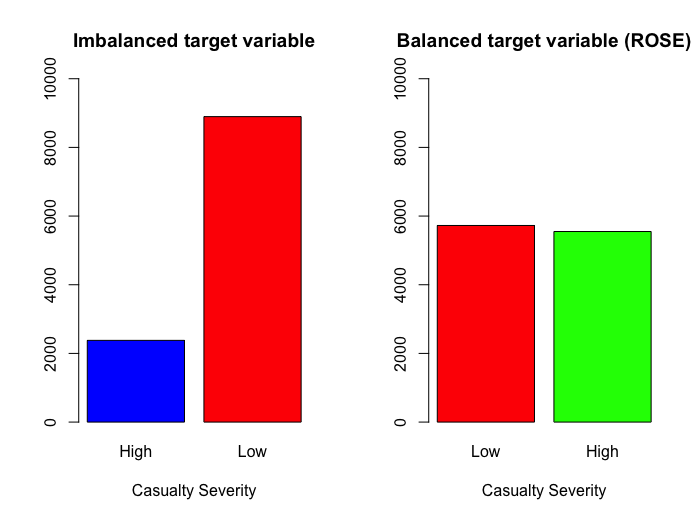
\includegraphics[width=0.75\linewidth]{rose} 

}

\caption{Comparison of the distribution of target variable after the implementation of ROSE technique}\label{fig:unnamed-chunk-16}
\end{figure}

(Figure 15) demonstrates the balancing of the target variable, `Casualty
Severity' using the ROSE (Random Over Sampling) technique. Thus, the
data is balanced for the training dataset.

\hypertarget{implementing-naive-bayes}{%
\subsection{Implementing Naive Bayes}\label{implementing-naive-bayes}}

The confusion Matrix shown in table 8 was built using naive bayes model
using package `caret' from r library (Kuhn (2020)) for (table 9) the
training dataset and (table 10) testing dataset respectively. From the
table 11 it can be seen that the model with testing dataset has higher
accuracy more than the training dataset.

\begin{table}[!htb]
    \caption{Confusion matrix of naive bayes model}
    \begin{minipage}{.5\linewidth}
      \caption{Training Set}
      \centering
        \begin{tabular}{lll}
        & Reference & \\
         Prediction  & Low & High\\
           Low & 2673 & 1982 \\
          High & 1330 & 1908  \\
        \end{tabular}
    \end{minipage}%
    \begin{minipage}{.5\linewidth}
      \centering
        \caption{Testing Set}
        \begin{tabular}{lll}
          & Reference & \\
          Prediction  & High & Low \\
           High & 49 & 54 \\
            Low & 670 & 2610\\
        \end{tabular}
    \end{minipage} 
\end{table}

\begin{table}[ht]
\caption{Summary of naive bayes model} 
\centering
\begin{tabular}{c@{\hskip 0.5in}c@{\hskip 0.5in}c@{\hskip 0.5in}c@{\hskip 0.5in}}
\hline\hline
Model & Accuracy & Precision & Recall \\ [0.5ex]
\hline
Train & 58.04\% & 57.42\% & 66.77\% \\ 
Test & 78.65\% & 47.57\% & 68.15\% \\[1ex]
\hline
\end{tabular}
\end{table}

\newpage

\hypertarget{implementing-logistic-regression}{%
\subsection{Implementing Logistic
Regression}\label{implementing-logistic-regression}}

The confusion Matrix shown in table 12 was built using logistic
regression model using package `mass' from r library (Venables and
Ripley (2002)) for (table 13) the training dataset and (table 14)
testing dataset respectively. From the table 15 it can be seen that the
model with training dataset has higher accuracy more than the testing
dataset.

\begin{table}[!htb]
    \caption{Confusion matrix of logistic regression model}
    \begin{minipage}{.5\linewidth}
      \caption{Training Set}
      \centering
        \begin{tabular}{lll}
        & Reference & \\
         Prediction  & Low & High\\
           Low & 2571 & 1432 \\
          High & 1791 & 2099  \\
        \end{tabular}
    \end{minipage}%
    \begin{minipage}{.5\linewidth}
      \centering
        \caption{Testing Set}
        \begin{tabular}{lll}
          & Reference & \\
          Prediction  & High & Low \\
           High & 16 & 703 \\
            Low & 7 & 2657\\
        \end{tabular}
    \end{minipage} 
\end{table}

\begin{table}[!htb]
\caption{Summary of logistic regression model} 
\centering
\begin{tabular}{c@{\hskip 0.5in}c@{\hskip 0.5in}c@{\hskip 0.5in}c@{\hskip 0.5in}}
\hline\hline
Model & Accuracy & Precision & Recall \\ [0.5ex]
\hline
Train & 59.16\% & 59.44\% & 53.95\% \\ 
Test & 20.98\% & 20.92\% & 97.77\% \\[1ex]
\hline
\end{tabular}
\end{table}

\hypertarget{implementing-decision-tree}{%
\subsection{Implementing Decision
Tree}\label{implementing-decision-tree}}

The confusion Matrix shown in table 16 was built using decision tree
model using package `rpart' from r library (Therneau and Atkinson
(2019)) for (table 17) the training dataset and (table 18) testing
dataset respectively. From the table 19 it can be seen that the model
with testing dataset has higher accuracy more than the training dataset
but the with no precision and a recall with a value 0.

\begin{table}[!htb]
    \caption{Confusion matrix of decision tree model}
    \begin{minipage}{.5\linewidth}
      \caption{Training Set}
      \centering
        \begin{tabular}{lll}
        & Reference & \\
         Prediction  & Low & High\\
           Low & 2204 & 1576 \\
          High & 1799 & 2314  \\
        \end{tabular}
    \end{minipage}%
    \begin{minipage}{.5\linewidth}
      \centering
        \caption{Testing Set}
        \begin{tabular}{lll}
          & Reference & \\
          Prediction  & High & Low \\
           High & 0 & 0 \\
            Low & 719 & 2664\\
        \end{tabular}
    \end{minipage} 
\end{table}

\begin{table}[ht]
\caption{Summary of decision tree model} 
\centering
\begin{tabular}{c@{\hskip 0.5in}c@{\hskip 0.5in}c@{\hskip 0.5in}c@{\hskip 0.5in}}
\hline\hline
Model & Accuracy & Precision & Recall \\ [0.5ex]
\hline
Train & 57.24\% & 58.31\% & 55.06\% \\ 
Test & 78.75\% & NAN\% & 0\% \\[1ex]
\hline
\end{tabular}
\end{table}

\newpage

\hypertarget{implementing-random-forest}{%
\subsection{Implementing Random
Forest}\label{implementing-random-forest}}

The confusion Matrix shown in table 20 was built using random forest
model using package `randomforest' from R library (Liaw and Wiener
(2002)) for (table 21) the training dataset and (table 22) testing
dataset respectively. From the table 23 it can be seen that the model
with training dataset has higher accuracy more than the testing dataset.

\begin{table}[!htb]
    \caption{Confusion matrix of random forest model}
    \begin{minipage}{.5\linewidth}
      \caption{Training Set}
      \centering
        \begin{tabular}{lll}
        & Reference & \\
         Prediction  & Low & High\\
           Low & 3953 & 103 \\
          High & 50 & 3787 \\
        \end{tabular}
    \end{minipage}%
    \begin{minipage}{.5\linewidth}
      \centering
        \caption{Testing Set}
        \begin{tabular}{lll}
          & Reference & \\
          Prediction  & High & Low \\
           High & 530 & 0 \\
            Low & 189 & 2664\\
        \end{tabular}
    \end{minipage} 
\end{table}

\begin{table}[!htb]
\caption{Summary of random forest model} 
\centering
\begin{tabular}{c@{\hskip 0.5in}c@{\hskip 0.5in}c@{\hskip 0.5in}c@{\hskip 0.5in}}
\hline\hline
Model & Accuracy & Precision & Recall \\ [0.5ex]
\hline
Train & 98.02\% & 97.46\% & 98.68\% \\ 
Test & 94.41\% & 1\% & 73.71\% \\[1ex]
\hline
\end{tabular}
\end{table}

\newpage
\begin{figure}[h!]

{\centering 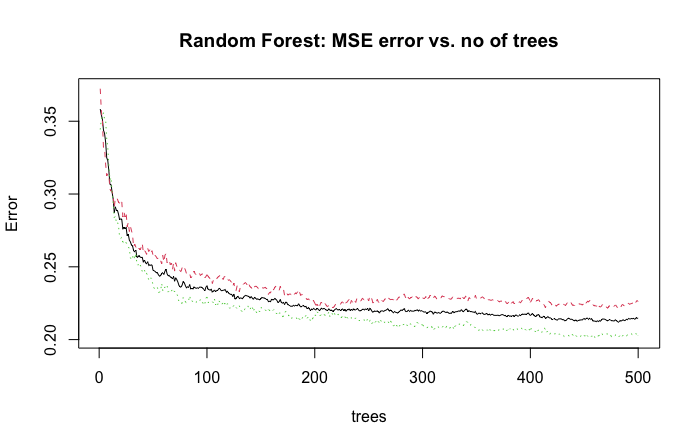
\includegraphics[width=0.55\linewidth]{mserf} 

}

\caption{Comparison of error vs. the no. of trees.}\label{fig:unnamed-chunk-17}
\end{figure}

Figure 16 shows how the error decreases with the increase in the number
of trees, after 300, the error rate is not much increasing which tends
to almost constant. As a result, the model was designed with 500 trees,
although the data set is wide and requires longer computation time for
better predictive performance.

\hypertarget{identifying-the-important-variables-from-random-forest-model}{%
\subsubsection{Identifying the important variables from random forest
model:}\label{identifying-the-important-variables-from-random-forest-model}}

The importance of each variable in the built-in model is calculated
using a random forest algorithm. The significance is calculated on the
basis of the mean decrease in the Gini coefficient. Gini coefficient is
a measure of how each attribute contributes to the homogeneity of the
nodes and results in the resulting random forest. Attributes that are
significant possesses a higher mean decrease in Gini coefficient. (Table
24) indicates the importance of each independent variable in the random
forest model.

\begin{table}[h]
\caption{Importance of each variables based on mean decrease in Gini.}
\bigskip
\centering
\begin{tabular}{l c}
\hline\hline
 & MeanDecreaseGini\\ [0.75ex]
\hline
Date                            &  516.29260\\
Day\_of\_Week                      & 353.78081\\
Time                              &212.39392\\
Road\_Type                       &  156.33193\\
Speed\_limit         &              166.68112\\
Junction\_Detail      &             282.16488\\
Junction\_Control      &             97.79726\\
Light\_Conditions       &            37.61521\\
Weather\_Conditions      &          114.76511\\
Road\_Surface\_Conditions  &          76.16405\\
Special\_Conditions\_at\_Site  &       21.24384\\
Urban\_or\_Rural\_Area          &      55.26323\\
Sex\_of\_Casualty               &     89.72172\\
Age\_of\_Casualty  &              681.05445\\
Journey\_Purpose\_of\_Driver     &     114.73173\\ [1ex]
\hline
\end{tabular}
\end{table}

As per (Figure 17), it is noted that, apart from the last 6 variables,
`Junction Control', `Sex of Casualty', `Road surface conditions', `Urban
or Rural Area', `Light conditions' and `Special Conditions at Site' all
the other variables have a mean decrease score of above 100. Such
variables are then defined as important for the model and are used as
the only input variable for another model. This model is free from the
contribution of the other 6 irrelevant variables.

\begin{figure}[h!]

{\centering 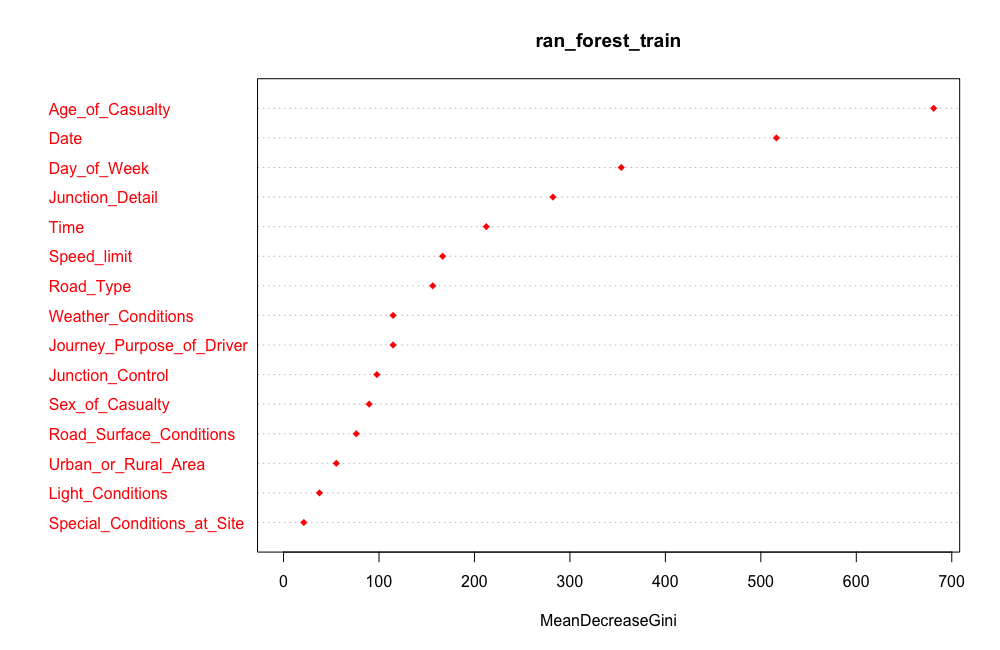
\includegraphics[width=0.75\linewidth]{varimp} 

}

\caption{Significance of the variables plotted based on mean decrease in Gini}\label{fig:unnamed-chunk-18}
\end{figure}

\hypertarget{implementing-all-models-with-only-the-identified-important-variables-as-input.}{%
\subsubsection{Implementing all models with only the identified
important variables as
input.}\label{implementing-all-models-with-only-the-identified-important-variables-as-input.}}

Important variables found are fed as input variables to all of the
algorithms listed above to see if they boost the accuracy of the
existing models. Nonetheless, based on the analysis, there was no
difference between them and the current ones.

\begin{table}[h]
\caption{ Accuracy of the revised models}
\centering
\begin{tabular}{l@{\hskip 0.5in}c@{\hskip 0.5in}c@{\hskip 0.5in}c@{\hskip 0.5in}} \hline\hline
 Models & Dataset & Accuracy & \\ [0.5ex]
\hline 
& Train & 58.38\% & (0.34\% increase)\\[-1ex]
\raisebox{1.5ex}{Naive Bayes} & Test & 78.89\% & (0.24\% increase)\\[1ex]
& Train & 58.75\% & (0.41\% decrease)\\[-1ex] \raisebox{1.5ex}{Logistic Regression} &  Test & 21.07\%&(0.09\% decrease)\\[1ex]
& Train & 99.08\% & (1.06\% increase)\\[-1ex] \raisebox{1.5ex}{Random Forest} & Test & 98.91\% & (4.5\% increase)\\[1ex]
& Train & 57.24\% &(same as above)\\[-1ex] \raisebox{1.5ex}{Decision Tree} & Test & 78.75\% & (same as above)\\[1ex]
\hline 
\end{tabular}
\end{table}

On the basis of the above findings, Objective D is clear that negligible
variables did not really affect the output of the current models,
because they did not affect the accuracy of the revised models thus did
not contribute much to the estimation of the dependent variable.

\hypertarget{evaluation-based-on-the-accuracy-of-each-model}{%
\subsubsection{Evaluation based on the accuracy of each
model}\label{evaluation-based-on-the-accuracy-of-each-model}}

During this step, models developed at the data modeling stage for the
testing data are evaluated and compared to each other to determine the
best prediction model for this analysis.

\begin{figure}[h!]

{\centering 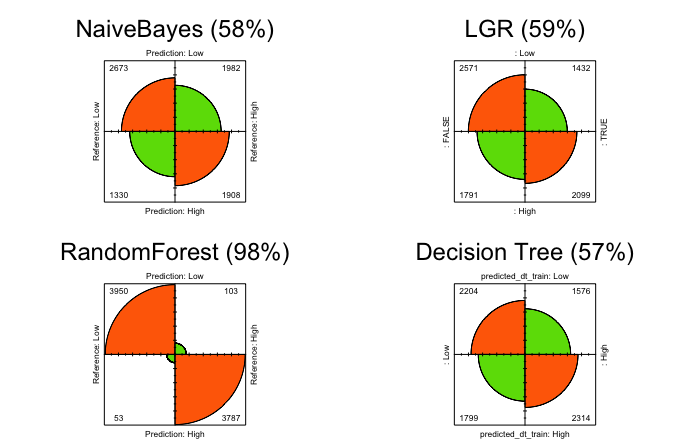
\includegraphics[width=0.75\linewidth]{fourfold train} 

}

\caption{Fourfold plot - comparison of all the models based on accuracy}\label{fig:unnamed-chunk-19}
\end{figure}

(Figure 18) displays the four-fold plot of all models, built on the
basis of their respective confusion matrixes using the balanced train
dataset. Based on their accuracy, the Random Forest model ranks at the
top with the highest accuracy of 98\%, followed by the logistic
regression model with an accuracy of 59\% , Naive Bayes with an accuracy
of 58\%. Model with the least accuracy of all is the Decision Tree model
with an accuracy of 57\%.

\hypertarget{evaluation-based-on-the-roc-curve-of-each-model}{%
\subsubsection{Evaluation based on the ROC curve of each
model}\label{evaluation-based-on-the-roc-curve-of-each-model}}

The ROC (Receiver Operating Characteristic) curve is a graphical plot
formed by plotting TP (True Positive) vs.~FP (False Positive). Effective
ROC curves should have a high AUC (area under curve) value. The higher
the AUC value, the better the model is. pROC library in r (Robin et al.
(2011)) was used to compute the ROC curves. (Figure 19) displays the ROC
curves of the models together with their AUC values. It is evident that
the Random Forest's ROC curve looks the best of all with highest AUC
value of 0.998 than other models.

\begin{figure}[h!]

{\centering 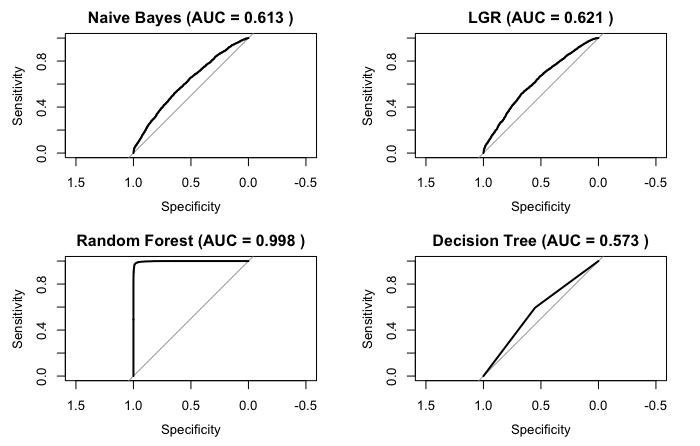
\includegraphics[width=0.75\linewidth]{roc} 

}

\caption{Comparison of  AUC values of all the models and ROC curves}\label{fig:unnamed-chunk-20}
\end{figure}

\newpage

\hypertarget{summary}{%
\subsubsection{Summary}\label{summary}}

Comparison of all four models using the balanced training set focused on
measures such as precision, accuracy, recall and AUC values. The
training dataset which consists of the balanced dataset performed well
than the testing dataset which was unbalanced. Thus objective C is being
clear of how to handle the imbalanced dataset. It is clear in both
training and test dataset that the Random Forest model excels in all the
metrics that make it the best model compared to all the other four
models, because it has achieved the highest metrics in all the
categories, whereas the Decision Tree has achieved the lowest values in
all the metrics. Thus objective B is being clear that random forest
performed well and is the most efficient algorithm. It means that the
precision of the model increases with the rise in the number of trees.
With the target variable levels, `casualty severity' being extremely
imbalanced, the models have performed fairly well. Table 26 displays the
summary of the training dataset and table 27 displays the summary of the
test dataset.

\begin{table}[!htb]
\caption{Summary of the training dataset table} 
\centering
\begin{tabular}{c@{\hskip 0.25in}c@{\hskip 0.25in}c@{\hskip 0.25in}c@{\hskip 0.25in}c@{\hskip 0.25in}}
\hline\hline
Model     & Accuracy(\%)    & Precision(\%)     & Recall(\%)    & AUC(\%) \\ [0.5ex]
\hline
Naive Bayes  &  58.04 & 57.42   & 66.77   & 0.613 \\
Logistic Regression    & 59.16    & 59.44     & 53.95 & 0.621 \\
Random Forest     & 98.02    & 97.46     & 98.69  & 0.998\\
Decision Tree & 57.24    & 58.31     & 55.06     & 0.573 \\ [1ex]
\hline
\end{tabular}
\end{table}

\begin{table}[!htb]
\caption{Summary of the testing dataset table} 
\centering
\begin{tabular}{c@{\hskip 0.25in}c@{\hskip 0.25in}c@{\hskip 0.25in}c@{\hskip 0.25in}c@{\hskip 0.25in}}
\hline\hline
Model     & Accuracy(\%)    & Precision(\%)     & Recall(\%)    & AUC(\%) \\ [0.5ex]
\hline
Naive Bayes  &  78.65 & 47.57   & 68.15   & 0.609 \\
Logistic Regression    & 20.98    & 20.92     & 97.77 & 0.616  \\
Random Forest     & 94.41   & 1     & 73.71  & 1\\
Decision Tree & 78.75    & NAN    & 0     &  0.5\\ [1ex]
\hline
\end{tabular}
\end{table}

\newpage

\hypertarget{conclusion-and-future-work}{%
\section{Conclusion and Future Work}\label{conclusion-and-future-work}}

The aim and purpose of this research project was to predict the severity
of cyclist accidents in the United Kingdom. Several data mining methods
have been used and tested to tackle the question of assessing the extent
of the accident in the United Kingdom. The machine learning algorithms
used for this study produced good results and addressed the research
question. Starting with data preparation, missing values were handled
and multiple classes that were ambiguous in each factor variable were
handled to have meaningful classes for better data analysis using
binning technique. The Random Oversampling (ROSE) technique was then
applied to manage the imbalanced dataset as it could lead to bias
predictions and incorrect results. It has improved the efficiency of the
models and produced efficient accuracy results. Due to the difference in
the target variable between the three classes, two classes were combined
into one for better data balancing. With the purpose of successful data
analysis, the behaviors and trends of each variable have been analyzed
in the data exploration. It offered valuable insights into the
occurrence of accidents. It was found that most of the casualties
happened during the daytime or well-lit conditions on dry/wet roads when
the weather was absolutely good with no strong winds. The cyclist
accidents which happened at the speed limit of 30 are the area where
special measure is to be taken as 30 speed limit is considered as the
safe, the speed limit can either be reduced to 20 or the lane for
cyclist should be widen to reduce the casualties. Several classification
models have been developed to allow an accurate prediction of the target
variable. It was observed that the Random Forest technique worked the
best of all the other models with a precision of 98\%. The work carried
out in this project, the applicant wants to carry out future research by
doing some time series analysis and using data from previous year to see
the month and time of accident in some areas which can help to see how
many cyclist casualties are affected in several years.

\newpage
\appendix
\section{Appendix}

This section contains plots for the unbalanced testing datasets.

--Significance of the variables plot for unbalanced test dataset.

\begin{figure}[h!]

{\centering 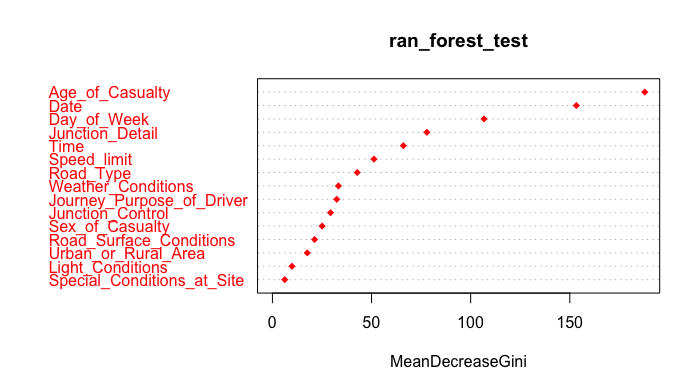
\includegraphics[width=0.6\linewidth]{testvarimp} 

}

\caption{Significance of the variables plotted based on mean decrease in Gini}\label{fig:unnamed-chunk-21}
\end{figure}

--Fourfold plot for unbalanced test dataset.

\begin{figure}[h!]

{\centering 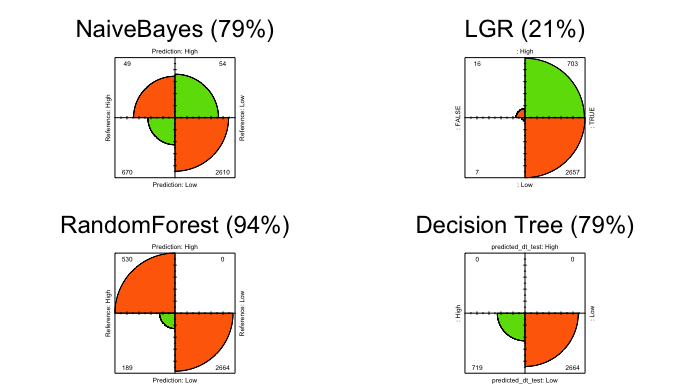
\includegraphics[width=0.6\linewidth]{testfourplot} 

}

\caption{Fourfold plot - comparison of all the models based on accuracy}\label{fig:unnamed-chunk-22}
\end{figure}

--Comparison of AUC values for unbalanced test dataset.

\begin{figure}[h!]

{\centering 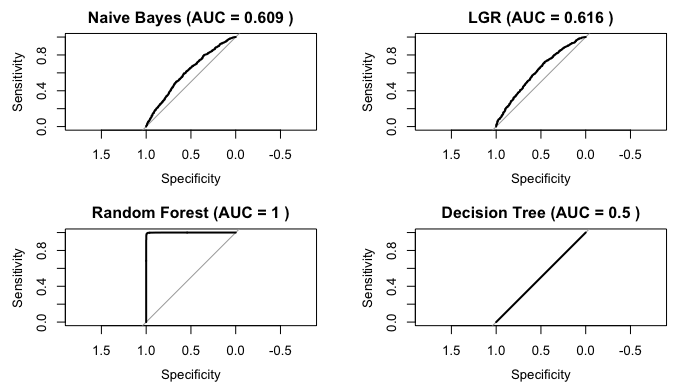
\includegraphics[width=0.6\linewidth]{testroc} 

}

\caption{Comparison of  AUC values of all the models and ROC curves}\label{fig:unnamed-chunk-23}
\end{figure}

\newpage
\newpage

\hypertarget{bibliography}{%
\section*{Bibliography}\label{bibliography}}
\addcontentsline{toc}{section}{Bibliography}

\hypertarget{refs}{}
\leavevmode\hypertarget{ref-7975380}{}%
Ahlawat, A., and B. Suri. 2016. ``Improving Classification in Data
Mining Using Hybrid Algorithm,'' 1--4.

\leavevmode\hypertarget{ref-ali}{}%
Ali Tavakoli Kashani, Afshin Shariat Mohaymany. 2017. ``Analysis of the
Traffic Injury Severity on Two-Lane, Two-Way Rural Roads Based on
Classification Tree Models.'' \emph{ELSEVIER} 49 (10): 1314--20.
\url{https://www.sciencedirect.com/science/article/pii/S092575351100110X}.

\leavevmode\hypertarget{ref-atnafu}{}%
Baye Atnafu, Gagandeep Kaur. 2017. ``Analysis and Predict the Nature of
Road Traffic Accident Using Data Mining Techniques in Maharashtra,
India.'' \emph{IJETSR} 4 (10).
\url{https://www.researchgate.net/profile/Baye_Atnafu/publication/325414837_Analysis_and_predict_the_nature_of_road_traffic_accident_using_data_mining_techniques_in_Maharashtra_India/links/5b0cc94d0f7e9b1ed7fbc754/Analysis-and-predict-the-nature-of-road-traffic-accident-using-data-mining-techniques-in-Maharashtra-India.pdf}.

\leavevmode\hypertarget{ref-matrix}{}%
Bengtsson, Henrik. 2020. \emph{MatrixStats: Functions That Apply to Rows
and Columns of Matrices (and to Vectors)}.
\url{https://CRAN.R-project.org/package=matrixStats}.

\leavevmode\hypertarget{ref-brennan}{}%
Brennan, Peter. 2012. ``A Comprehensive Survey of Methods for Overcoming
the Class Imbalance Problem in Fraud Detection.'' PhD thesis.
\url{https://doi.org/10.13140/RG.2.1.3375.5284}.

\leavevmode\hypertarget{ref-blower}{}%
Daniel Blower, Paul E.Green, Kenneth L.Campbell. 1993. ``Accident Rates
for Heavy Truck-Tractors in Michigan.'' \emph{ELSEVIER} 25 (3): 307--21.
\url{https://www.sciencedirect.com/science/article/pii/000145759390025R}.

\leavevmode\hypertarget{ref-7492647}{}%
Datla, M. V. 2015. ``Bench Marking of Classification Algorithms:
Decision Trees and Random Forests - a Case Study Using R,'' 1--7.

\leavevmode\hypertarget{ref-e1071}{}%
Dimitriadou, Evgenia, Kurt Hornik, Friedrich Leisch, David Meyer,
Andreas Maintainer, friedrich Leisch@ci, Ac Tuwien, and At. 2006. ``The
E1071 Package,'' August.

\leavevmode\hypertarget{ref-omit}{}%
Dowle, Matt, and Arun Srinivasan. 2019. \emph{Data.table: Extension of
`Data.frame`}. \url{https://CRAN.R-project.org/package=data.table}.

\leavevmode\hypertarget{ref-zong}{}%
Fang Zong, Hongguo Xu, and Huiyong Zhang. 2013. ``Prediction for Traffic
Accident Severity: Comparing the Bayesian Network and Regression
Models.'' \emph{Hindawi Publishing Corporation} 94 (6): 89--98.
\url{http://downloads.hindawi.com/journals/mpe/2013/475194.pdf}.

\leavevmode\hypertarget{ref-caret}{}%
Kuhn, Max. 2020. \emph{Caret: Classification and Regression Training}.
\url{https://CRAN.R-project.org/package=caret}.

\leavevmode\hypertarget{ref-7965753}{}%
Li, L., S. Shrestha, and G. Hu. 2017. ``Analysis of Road Traffic Fatal
Accidents Using Data Mining Techniques.'' In \emph{2017 Ieee 15th
International Conference on Software Engineering Research, Management
and Applications (Sera)}, 363--70.

\leavevmode\hypertarget{ref-random}{}%
Liaw, Andy, and Matthew Wiener. 2002. ``Classification and Regression by
randomForest.'' \emph{R News} 2 (3): 18--22.
\url{https://CRAN.R-project.org/doc/Rnews/}.

\leavevmode\hypertarget{ref-stats}{}%
Lovelace, Robin, Malcolm Morgan, Layik Hama, Mark Padgham, David
Ranzolin, and Adam Sparks. 2019. ``Stats 19: A Package for Working with
Open Road Crash Data.'' \emph{The Journal of Open Source Software} 4
(33): 1181. \url{https://doi.org/10.21105/joss.01181}.

\leavevmode\hypertarget{ref-Informatica}{}%
Miao Chong, Ajith Abraham, and Marcin Paprzycki. 2005. ``Traffic
Accident Analysis Using Machine Learning Paradigms.'' \emph{Informatica
29} 94 (6): 89--98.
\url{http://wsc9.softcomputing.net/informatica2.pdf}.

\leavevmode\hypertarget{ref-zekic}{}%
M. Zekić-Sušac, A. Has, N. Šarlija, and A. Bilandžić. 2016. ``Predicting
Company Growth Using Logistic Regression and Neural Networks.''
\emph{Croatian Operational Research Review} 7 (2): 229--48.
\url{https://doi.org/10.17535/crorr.2016.0016}.

\leavevmode\hypertarget{ref-rose}{}%
Nicola Lunardon, Giovanna Menardi, and Nicola Torelli. 2014. ``ROSE: A
Package for Binary Imbalanced Learning.'' \emph{The R Journal} 6 (1):
79--89.
\url{https://journal.r-project.org/archive/2014/RJ-2014-008/RJ-2014-008.pdf}.

\leavevmode\hypertarget{ref-harb}{}%
Rami Harb, Essam Radwan, Xuedong Yan. 2009. ``Exploring Precrash
Maneuvers Using Classification Trees and Random Forests.''
\emph{ELSEVIER} 41 (1): 98--107.
\url{https://www.sciencedirect.com/science/article/pii/S0001457508001887}.

\leavevmode\hypertarget{ref-proc}{}%
Robin, Xavier, Natacha Turck, Alexandre Hainard, Natalia Tiberti,
Frédérique Lisacek, Jean-Charles Sanchez, and Markus Müller. 2011.
``PROC: An Open-Source Package for R and S+ to Analyze and Compare Roc
Curves.'' \emph{BMC Bioinformatics} 12: 77.

\leavevmode\hypertarget{ref-ukgov}{}%
Safety, UK Road. 2018. ``Department for Transport.''
\url{http://data.gov.uk}.

\leavevmode\hypertarget{ref-Sowmya}{}%
Sowmya, and P. Ponmuthuramalingam. 2013. ``Analyzing the Road Traffic
and Accidents with Classification Techniques.'' In.

\leavevmode\hypertarget{ref-shanthi}{}%
S. Shanthi, R. Geetha Ramani. 2012. ``Feature Relevance Analysis and
Classification of Road Traffic Accident Data Through Data Mining
Techniques.'' \emph{WCECS} 1.
\url{http://www.iaeng.org/publication/WCECS2012/WCECS2012_pp122-127.pdf}.

\leavevmode\hypertarget{ref-rpart}{}%
Therneau, Terry, and Beth Atkinson. 2019. \emph{Rpart: Recursive
Partitioning and Regression Trees}.
\url{https://CRAN.R-project.org/package=rpart}.

\leavevmode\hypertarget{ref-mass}{}%
Venables, W. N., and B. D. Ripley. 2002. \emph{Modern Applied Statistics
with S}. Fourth. New York: Springer.
\url{http://www.stats.ox.ac.uk/pub/MASS4}.

\leavevmode\hypertarget{ref-tidyverse}{}%
Wickham, Hadley, Mara Averick, Jennifer Bryan, Winston Chang, Lucy
D'Agostino McGowan, Romain François, Garrett Grolemund, et al. 2019.
``Welcome to the tidyverse.'' \emph{Journal of Open Source Software} 4
(43): 1686. \url{https://doi.org/10.21105/joss.01686}.

\end{document}
